\documentclass[11pt]{article}
\usepackage{setspace}
\usepackage{hyperref}
\usepackage[utf8]{inputenc}
\usepackage[T1]{fontenc}
\usepackage{fullpage}
\usepackage{amsmath}
\usepackage{amssymb,amsfonts}
\usepackage[all,arc]{xy}
\usepackage{enumerate}
\usepackage{mathrsfs}
\usepackage{bbm}
\usepackage{graphicx}
\usepackage{subfiles}
\usepackage{setspace}
\usepackage{float}
\usepackage{subcaption}
\usepackage{verbatim}
\usepackage{listings}
\usepackage{wrapfig}
\setlength{\footskip}{40pt}
\graphicspath{{Figures/}}
\numberwithin{figure}{section}
\setlength\parindent{0pt}

\begin{document}
	\begin{center}
		\textsc{\Large{A Proposal for Policy Decisions and Phase Definitions \\}}
		\textsc{Ariel Hoffman \\}
		\hrulefill 
	\end{center}
	\section{\textsc{The Big Picture}}
		The main objective of this project is to determine a way to dynamically optimize a storage array by predicting workload patterns. The current system is described in Figure 1.1 (sans the red lines). It works as follows: first, the current state of the storage array is evaluated by the state categorizer (using something like K-means clustering or LoadIQ). The state categorizer tells the prediction model the current state. The prediction model stores previous states and the current state and then, using some prediction scheme (like C-Miner, Markhov Chains, or some combination) it estimates the next state's workload. It then passes that information to the array tuner as a set of features. The array tuner uses the predicted features to determine how it should tune the storage array. Currently the set of features is exclusively the LBA access pattern in the form of a histogram.\\
		
		\begin{wrapfigure}{r}{0.5\textwidth}
			\caption{Optimizer Diagram}
			\centering
			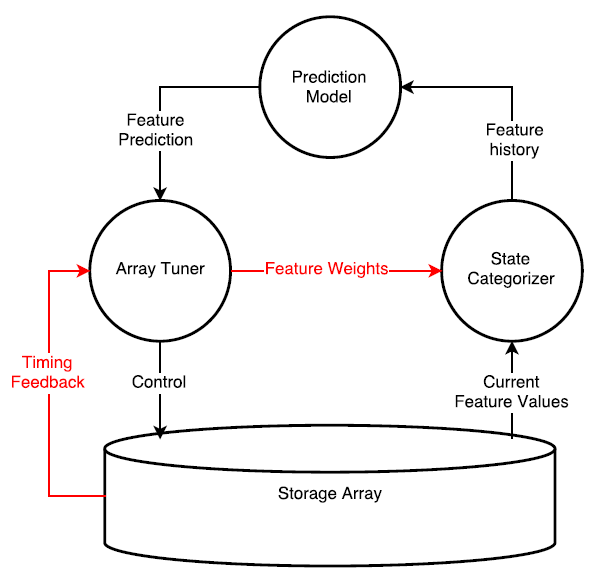
\includegraphics[width=0.5\textwidth]{BigPicture.png}
		\end{wrapfigure}
		
		This paper makes two proposals:
		\begin{enumerate}
			\item A proposal for an unsupervised storage array tuner that uses Temporal Difference Learning to determine what the best policies should be by accounting for live timing feedback.
			\item A proposal for an autonomous state categorizer that uses feedback from the array tuner in order to categorize states based on the features that actually matter most to performance.
		\end{enumerate}
		The key to understanding this proposal is to remember that the features stay the same throughout this diagram, but the abstract definition of state can improve over time as the array tuner provides better and better feedback about the importance of each feature. The array tuner decides what features are important based on feedback from the storage array and then it sends that information to the state categorizer. The state categorizer then uses all the information it has collected about previous states and it redefines its distance metric based on the feature weights provided by the array tuner. As a result, the prediction model will get better at providing data to the array tuner (because its states will be defined based on the important features) which will, in turn, become more precise. \\
		
		The main reason we investigate this approach is that our current feature is not sufficient for distinguishing between states effectively. We are currently only using the LBA access histogram as a feature and, even on clearly periodic traces, it is not giving us the desired resolution of data. The mechanism outlined herein allows us to naively give the system data and the system itself can adapt to determine the most important features.\\
		
		The main advantage of this proposal would be as follows:
		\begin{enumerate}
			\item A low-maintenence learning system that can autonomously identify important features. It can tune itself so that the whole system is sensitive to those features as well. 
			\item Better performance than a system that only takes advantage of the LBA histogram.
		\end{enumerate}
		
		The main risks associated with this study are as follows:
		\begin{enumerate}
			\item We may not be able to find any features that sufficiently encapsulate the important attributes of the phases.
			\item If we do find those features, the training phase may not converge on those features as important.
			\item It might turn out that the training phase takes too long. That said, our current setup is essentially this system with a single feature. Therefore, I believe that this system will not be any worse than what we would be producing otherwise.
			\item The main proponent of this idea (myself) is still in school and has significantly less experience than most people in this field. Therefore, there is a significant possibility that there are aspects of the problem that haven't been accounted for.
		\end{enumerate}
		
		The rest of this paper will be devoted to detailing the technical portions of the idea. Section 2 will provide a brief introduction to the math behind temporal difference learning. Section 3 will show how that math applies to the cache by defining the stage and the cost in context and giving some examples of features. Section 4 is a brief non-technical discussion on providing feedback to the state categorizer and why that is important. Section 5 is a psuedocode description of this system. 

	\section{\textsc{A Brief Introduction to Temporal Difference Learning}}		
		In dynamic programming, \textbf{cost to go} is used in order to determine what the optimal next state should be. We can do this because we can define the current cost to go recursively with respect to the next cost to go: the current cost to go is the next cost to go plus the transition cost.
		\begin{equation}
		J^*_k(x_k)=g(x_k,u_k)+J^*_{k+1}(x_{k+1})
		\end{equation}
		It is then possible to compute the minimal cost by starting from the end states and working backwards. The end state of a system must be associated with a set cost to go because there are no more actions to be made. Therefore, \begin{math}J^*_N(x_N)=g(x_N)\end{math}. If the number of possible \begin{math}x_N\end{math} is small enough, it is computationally possible to iterate through all possible values and work backwards for each of them. However, in games like Tetris and in our system, the reward to go (the negative cost to go) is impossible to calculate because the state space is too large. Therefore, to take advantage of dynamic programming, we must use approximations of the cost to go. We can do this using a set of features and a set of feature weights. \\
		
		When designing features to use in dynamic programming, it is not important what kind of impact the features have on the outcome because the system will dynamically modify the weights according to a feedback system. That said, the feature designer should try to design features that are relevant to the ultimate outcome of the system in order to reduce training time. In the case of Tetris, good features might include the height of the highest column or the difference between the height of the highest column and the hight of the lowest column. This is because these attributes will likely have a significant impact on the duration of the game and the points accrued along the way. When we're evaluating the state of the cache simulator, we will have to make features that include information about the policies and the contents of the trace. Eventually, we might even consider including information about the cache contents, though that seems unnecessary at this point. \\
		
		We should create a number of these features and we should store them in a vector, \begin{math}\phi^T\end{math}. Then, in order to approximate \begin{math}J(x_k)\end{math} (the cost or reward to go) we can use the following equation where \begin{math}x_k\end{math} represents a state, \begin{math}\phi^T(x_k)\end{math} represents the feature vector for the state, and \begin{math}r\end{math} represents a vector of predefined feature weights:
		\begin{equation}
			J(x_k) = \phi^T(x_k)r
		\end{equation}
		
		After creating an initial model, it is important to implement a feedback system so that that model can improve. To do this, one must compute the \textbf{temporal difference}. The temporal difference is simply the difference between the estimated transition cost (the estimated cost to go at the current state minus the estimated cost to go at the next state) \begin{math}\phi^T(x_k)r_k - \phi^T(x_{k+1})r_k\end{math} and the real transition cost, \begin{math}g(x_k,u_k)\end{math}.
		\begin{equation}
		d_k=g(x_k,u_k)+\phi^T(x_{k+1})r_k-\phi^T(x_k)r_k
		\end{equation}
		(Note well, for a perfect model, this value would always be zero.)
		After computing the temporal difference, one must adjust feature weights appropriately to make the model more accurate. To do this, one must compute the unit direction vector of the feature vector as follows:
		\begin{equation}
		z_t=\frac{\phi(x_t)}{||\phi(x_t)||}
		\end{equation}
		
		Next, one must simply apply the following equation to modify the feature weight vector:
		\begin{equation}
		r_{t+1}=r_t+\gamma_td_kz_t
		\end{equation}
		
		Where \begin{math}\gamma_t\end{math} is a tunable decaying constant. The decaying constant is important to diminish the impact of new data points during later stages. Often times this decaying constant is \begin{math}\frac{1}{\sqrt{k})}\end{math}, where \begin{math}k\end{math} is the current stage. \\
		
		After running this improvement algorithm many times, the \begin{math}r\end{math} values will eventually converge. This will allow the system to quickly decide what the next best state should be (and therefore, which policies we should implement.)
		
	\section{\textsc{Applications in Caching}}
		\subsection{Stages}
			Every stage can be defined as an interval of commands. Let the number of commands in each stage be \begin{math}q\end{math}. Thus, the commands issued between 0 and \begin{math}q\end{math} will be part of stage 0 and the commands issued between \begin{math}q\end{math} and \begin{math}2q\end{math} will belong to stage 1 and so on. Let the current stage be \begin{math}k\end{math}. If \begin{math}c\end{math} represents total number of commands issued until now, the current stage can therefore be calculated as follows:
			\begin{equation}
			k=floor(\frac{c}{q})
			\end{equation}
		\subsection{Features}
			In this setting, the features should be the sorts of things we think are likely to impact the effectiveness of a particular policy. So, for instance, suppose we are trying to determine whether a cache should be set to operate as
			\begin{enumerate}
				\item a write back cache
				\item a write through cache
				\item a write around cache
				\item no cache
			\end{enumerate}
			and we suspect that the following features are relevant to the outcome of the optimization problem:
			\begin{enumerate}
				\item the projected percent reads
				\item the projected percent writes
				\item the projected hit ratio
				\item the projected miss ratio
			\end{enumerate}
			We will be storing a weight associated with the impact of each feature given a different policy decision. Suppose our weights are defined as follows:
			$$
			W=
			\begin{bmatrix}
			r_{11}&r_{12}&r_{13}&r_{14}\\
			r_{21}&r_{22}&r_{23}&r_{24}\\
			r_{31}&r_{32}&r_{33}&r_{34}\\
			r_{41}&r_{42}&r_{43}&r_{44}\\
			\end{bmatrix}
			$$
			And the projected features are:
			$$
			f=
			\begin{bmatrix}
			f_{1}\\
			f_{2}\\
			f_{3}\\
			f_{4}\\
			\end{bmatrix}
			$$
			Then the policy index is simply the column-wise minimum of the product of \begin{math}Wf\end{math}:
			\begin{equation}
			policy = arg\min_i (r_{i1} f_1+r_{i2} f_2 + r_{i3} f_3 + r_{i4} f_4)
			\end{equation}
			Or, written in matrix form taking advantage of basis vectors (all elements are 0 except the ith element, which is 1), we have
			\begin{equation}
			policy = arg\min_i(Wfe_i)
			\end{equation}
			This is the example of a single policy choice. In our case, we will have multiple policy choices and they will all follow roughly the same pattern. Each will need to be minimized in turn.
		\subsection{Cost}
			Because this is a real system, the transition cost is the time it takes to complete the phase. If \begin{math}u_k\end{math} is the selected action, then
			\begin{equation}
			g(x_k, u_k)=time
			\end{equation}
		\subsection{Example Iteration}
			The state categorizer will have a whole history of states to work with. It will use an initial r vector in order to define a "distance" metric. Then, using some algorithm (LoadIQ, K-Means Clustering, etc.) it will put the current state into a category. Next, the state predictor will use the history of states provided by the categorizer as well as the current state to estimate the upcoming state. The state will be associated with a set of attributes. The temporal difference learner will look up these values (in this case, the number of writes and reads) and it will use the current \textit{r} value to determine the best next possible states. Suppose the predictor predicts that the next phase will have 70\% reads and 30\% writes. Because the system can control policy but not the attributes of the workload, there are only have two possible next states: either the system turns on the read cache or the system turns off the read cache. The system can calculate an approximately optimal time to completion using our features and our weightings as follows:
			\begin{math}
			J^*_k=\phi(x_{k+1})=\min\limits_{p}([f_1, f_2]^T*[r_1, r_2])
			\end{math}
			
			So, the algorithm makes the following decision:
			\begin{equation}
				p=
				\begin{cases}
				1 & hpr_1+mpr_2>0 \\
				0 & hpr_1+mpr_2\leq0
				\end{cases}
			\end{equation}
			
			It is worth noting again that the above solution does not necessarily produce the optimal value. However, by tuning the algorithm, the system can approach the optimal value using feedback. This process involves three steps:
			\begin{enumerate}
				\item Calculate \begin{math}\phi^T(x_{k+1})\end{math}: because time has passed and  \begin{math}x_{k+1}\end{math} is known with certainty, we can calculate the feature vector for it.
				\item Record \begin{math}g(x_k, u_k)\end{math}: this is simply the time it took to complete the phase.
				\item Calculate \begin{math}d_k\end{math}: we have already computed \begin{math}\phi^T(x_{k})\end{math}, so computing \begin{math}d_k\end{math} is merely a matter of using equation 3.
				\item Calculate \begin{math}z_t\end{math} using equation 4. 
				\item Calculate the new \begin{math}r_{t+1}\end{math} using equation 5.
			\end{enumerate}
			This process can be repeated again and again until r converges.
	\section{\textsc{Providing Feedback to the State Categorizer}}
		No matter what state categorizer is implemented, it will require a definition of distance. This definition of distance will invariably rely on the feature values. As a feedback mechanism, we should multiply these features by the weights computed by temporal difference learning. This will not alter the values of the features themselves, but it will alter the distances slightly.\\
		
		So, for instance, suppose we initially provided our temporal difference learning algorithm access to the number of times our workload accessed a specific data point. However, suppose that feature does not actually impact the performance of the system. First, the temporal difference learning algorithm will learn to ignore it. Next, the temporal difference learning algorithm will tell the state categorizer to ignore it as well so that the state categorizer can become more sensitive to ther attributes.
	\section{\textsc{Big Picture Pseudocode}}
		This section provides a more precise view of the big picture system. This psuedocode is not about the temporal difference learning, but rather the overall mechanism described in figure 1.1.
		\begin{scriptsize}
		\begin{lstlisting}
// Initial values
// My guess is that these will be a vector of 0s and 1s (i.e. on or off)
policyChoices = array of vectors of policy choices 
// see the discussion of features for a more detailed description
featureMatrix = matrix of features associated with each policy 
expertWeightings = initial value 
phaseModel = initial value
phasePredictionModel = initial value

// This function makes a guess about what the optimal next policy should be.
// The current feature matrix is known - it comes from the state 
// of the cache or the state of the array.
// The estimated next feature matrix will have to be determined by
// our predictive algorithm based on our phase definition.
function makeGuess(currentFeatureMatrix, estimatedNextFeatureMatrix):
	// This is deterministic - it's based on known features of the
	// cache and the trace we've already seen.
	currentCostToGo = calculateCurrentFeatureMatrix(this.cacheState)* \ 
		this.cacheState.currentPolicies

	// We want to find our minimum cost estimate.
	minimumEstimate = MAX_NUM
	for policyChoice in policyChoices:
		expertGuesses = estimatedNextFeatureMatrix*policyChoices
		estimatedCostToGo = expertGuesses*expertWeightings
		// Store whichever is smaller.
		if(estimatedCostToGo < minimumEstimate):
			minimumEstimate = estimatedCostToGo
			minimumPolicy = policyChoice
	assert minimumPolicy
	
	// Now that we have our minimum policy, we reinitialize
	// the cache accordingly
	initializeCache(minimumPolicy);

// In order to get our estimated next feature matrix, we need to use
// our model generated in C-miner or using standard Markhov chains
// to estimate what the next set of features will be. Basically we'll
// store a bunch of phases (like we're doing now) and those phases
// will have ideal feature matrix footprints (which is essentially what
// we're doing now, except with different features).
function getEstimatedNextFeatureMatrix(phaseModel, recentHistory):
	return phaseModel.getNextFeatureMatrix(recentHistory)

// This is the main training algorithm.
function trainModel:
	stateHistory = []
	while workloadRunning:
		// Here I choose 1000 as a reasonable number of phases to
		// run, but this is tunable.
		for i in xrange(1000):
			// We wait for our current phase to be available
			wait(cacheState.newPhaseInterrupt())
			
			// Get our current feature matrix
			currentFeatureMatrix = \
				calculateCurrentFeatureMatrix(this.cacheState)
			
			// keep a history of up to 1000 states
			// Note: this is not all the data; this is just the
			// data from the current feature matrix.
			// This will help us when we're remodelling stuff later.
			stateHistory = [stateHistory, currentFeatureMatrix]
			
			// Based on the model loadIQ created during its last run,
			// we sort this into a phase. This is analogous to what
			// we were doing with the histogram, except instead of
			// a histogram, we're dealing with a broader set of
			// featurs.
			currentPhase = \
				phaseModel.getCurrentPhase(currentFeatureMatrix);
			
			// Now, using the prediciton model, we guess about the
			// next phase. This could be a call to C-Miner or
			// Markhov chains or something
			nextPhaseGuess = \
				phasePredicitonModel.getNextPhaseGuess(currentFeatureMatrix);
			
			// Now that we have an idea of what our next phase
			// will be, we can figure out a good set of policies
			// using the algorithm described in the function makeGuess.
			makeGuess(currentFeatureMatrix, nextPhaseGuess.featureMatrix)
		
		// This should give us a model of "phases" so that during our next
		// round, we can start evaluating things based on what phase they
		// should belong to. Thinking about it now, this probably shouldn't
		// be loadIQ. This should be some other, independent algorithm. Take
		// careful note of the fact that we're feeding back our feature 
		// weightings into this algorithm. We do this because we want to
		// refine our definitons of the states so that they are more useful
		// when we're trying to decide on policies.
		phaseModel = loadIQ(stateHistory, featureWeightings)
		
		// Because we've recreated our phase model, we need to resort our phases
		// based on their feature matrices. (This is the reason we stored them 
		// away before.) This means that all the labels change. Because all the
		// labels have changed, we need to recreate our predictive model. This
		// resorts all the phases and adjusts our predictive model accordingly.
		phasePredictionmodel = cminer(stateHistory, phaseModel)
		\end{lstlisting}
		\end{scriptsize}
\end{document}